\documentclass[16pt]{article}
\usepackage[utf8]{inputenc}
\usepackage[T2A]{fontenc}
\usepackage[english, russian]{babel}
\usepackage{geometry}
\geometry{a4paper, left=30mm, right=15mm, top=20mm, bottom=20mm}
\usepackage{graphicx}
\usepackage{subcaption}
\usepackage{hyperref}
\usepackage{caption}

\begin{document}

\begin{titlepage}
    \begin{center}
        \large
        Санкт-Петербургский политехнический университет Петра Великого \\
        Институт машиностроения, материала и транспорта \\
        Федеральное государственное автономное образовательное учреждение \\
        Высшая школа автоматизации и робототехники \\

        \vspace{5cm}

        \textbf{Курсовая работа} \\
        \vspace{1cm}

        \textbf{Дисциплина: Объектно-ориентированное программирование} \\
        \textbf{Тема: Разработка ПЛК} \\

        \vspace{5cm}

        \begin{flushright}
            \large
            \textbf{Выполнил студент гр. 3331506/20401} \\
            Вчерашний З. Д. \\
            \textbf{Преподаватель} \\
            Ананьевский М. С. \\
        \end{flushright}

        \vfill

        Санкт-Петербург \\
        \the\year
    \end{center}
\end{titlepage}


\tableofcontents

\newpage
\section{Введение}
Современные промышленные системы, объединяющие алгоритмы технического зрения и нейронные сети, часто сталкиваются с проблемой архитектурной фрагментации из-за разделения функциональных модулей. Обычно такие системы состоят из нескольких ключевых компонентов:
\begin{enumerate}
    \item Специализированный модуль обработки изображений, выполняющий задачи обнаружения и классификации объектов;
    \item Контроллер, предназначенный для сбора данных с различных датчиков через интерфейсы, такие как UART, I2C и CAN;
    \item Промежуточные узлы, обеспечивающие предварительную обработку сигналов и преобразование интерфейсов.
\end{enumerate}

\section{Обзор литературы}
Интеграция нейросетевых моделей в промышленные системы активно изучается в рамках задач автоматизации, где ведутся разработки нейросетевых регуляторов для существующих программируемых логических контроллеров (ПЛК) \cite{ref1,ref2,ref3}. Исследования \cite{ref4,ref5} демонстрируют эффективность моделей YOLO и ResNet для обнаружения объектов на производственных линиях. Другие работы \cite{ref6,ref7} подчеркивают значимость аппаратного ускорения, например, с использованием технологий, таких как TensorRT.

\section{Расчет толщины дорожки и дренаж земляного полигона}

\subsection{Толщина дорожки в зависимости от тока}

Для расчета ширины дорожки на печатной плате используется следующая формула:

\[ w = \frac{I}{k \cdot \Delta T^b} \]

где \( w \) — ширина дорожки, \( I \) — ток, \( k \) и \( b \) — константы, зависящие от материала платы, а \( \Delta T \) — допустимое повышение температуры.

\subsection{Дренаж земляного полигона}

Дренаж земляного полигона на печатной плате важен для обеспечения стабильного заземления и минимизации помех. Основные принципы включают:

\begin{itemize}
    \item Минимизация импеданса заземления.
    \item Разделение аналогового и цифрового заземления.
    \item Учет тепловых характеристик.
\end{itemize}

\section{Сборка ядра Linux и загрузчика U-Boot}

\subsection{Подготовка окружения}

Перед началом сборки необходимо подготовить окружение, установив все необходимые инструменты и зависимости. Обычно это включает компилятор, утилиты для сборки и библиотеки.

\begin{itemize}
    \item Установка необходимых пакетов:
    \begin{verbatim}
    sudo apt-get update
    sudo apt-get install build-essential bc libncurses-dev flex bison libssl-dev
    \end{verbatim}
\end{itemize}

\subsection{Получение исходных кодов}

Необходимо получить исходные коды ядра Linux и загрузчика U-Boot. Это можно сделать, клонировав официальные репозитории с помощью Git.

\begin{itemize}
    \item Клонирование ядра Linux:
    \begin{verbatim}
    git clone https://git.kernel.org/pub/scm/linux/kernel/git/torvalds/linux.git
    \end{verbatim}

    \item Клонирование U-Boot:
    \begin{verbatim}
    git clone https://git.denx.de/u-boot.git
    \end{verbatim}
\end{itemize}

\subsection{Конфигурация ядра Linux}

После получения исходных кодов необходимо сконфигурировать ядро Linux в соответствии с требованиями вашей аппаратной платформы.

\begin{itemize}
    \item Переход в директорию с исходниками ядра:
    \begin{verbatim}
    cd linux
    \end{verbatim}

    \item Запуск конфигурации:
    \begin{verbatim}
    make menuconfig
    \end{verbatim}
\end{itemize}

\subsection{Сборка ядра Linux}

После конфигурации можно приступить к сборке ядра.

\begin{itemize}
    \item Запуск процесса сборки:
    \begin{verbatim}
    make -j$(nproc)
    \end{verbatim}
\end{itemize}

\subsection{Конфигурация U-Boot}

Аналогично ядру, необходимо сконфигурировать U-Boot для вашей аппаратной платформы.

\begin{itemize}
    \item Переход в директорию с исходниками U-Boot:
    \begin{verbatim}
    cd u-boot
    \end{verbatim}

    \item Запуск конфигурации:
    \begin{verbatim}
    make menuconfig
    \end{verbatim}
\end{itemize}

\subsection{Сборка U-Boot}

После конфигурации можно собрать U-Boot.

\begin{itemize}
    \item Запуск процесса сборки:
    \begin{verbatim}
    make -j$(nproc)
    \end{verbatim}
\end{itemize}

\subsection{Установка ядра и загрузчика}

После успешной сборки необходимо установить ядро и загрузчик на целевую систему.

\begin{itemize}
    \item Копирование ядра и загрузчика на целевую систему:
    \begin{verbatim}
    scp arch/arm/boot/zImage user@target:/boot/
    scp u-boot.bin user@target:/boot/
    \end{verbatim}
\end{itemize}

\subsection{Настройка загрузчика}

Последний этап включает настройку загрузчика для загрузки нового ядра.

\begin{itemize}
    \item Настройка U-Boot для загрузки ядра:
    \begin{verbatim}
    setenv bootcmd 'fatload mmc 0:1 0x80007fc0 zImage; bootz 0x80007fc0'
    saveenv
    \end{verbatim}
\end{itemize}


\section{Конфигурация библиотек Libmodbus и libcan для работы с аппаратными портами}

\subsection{Установка библиотек}

Для работы с аппаратными портами через протоколы Modbus и CAN необходимо установить соответствующие библиотеки. Ниже приведены инструкции по установке и базовой настройке.

\subsubsection{Установка Libmodbus}

Libmodbus — это библиотека, которая позволяет взаимодействовать с устройствами через протокол Modbus. Установка библиотеки может быть выполнена с помощью следующих команд:

\begin{verbatim}
sudo apt-get update
sudo apt-get install libmodbus-dev
\end{verbatim}

\subsubsection{Установка libcan}

Для работы с CAN-интерфейсами может потребоваться библиотека, такая как SocketCAN. Установите необходимые пакеты с помощью следующих команд:

\begin{verbatim}
sudo apt-get update
sudo apt-get install can-utils libsocketcan-dev
\end{verbatim}

\subsection{Конфигурация Libmodbus}

\subsubsection{Настройка соединения}

Для настройки соединения с устройством через Modbus необходимо указать параметры соединения, такие как адрес устройства, скорость передачи данных и другие параметры. Пример настройки соединения:

\begin{verbatim}
#include <modbus.h>
modbus_t *ctx;

ctx = modbus_new_rtu("/dev/ttyUSB0", 9600, 'N', 8, 1);
modbus_connect(ctx);
\end{verbatim}

\subsubsection{Чтение и запись данных}

Пример чтения и записи данных с использованием Libmodbus:

\begin{verbatim}
uint16_t tab_reg[64];

modbus_read_registers(ctx, 0, 10, tab_reg);
modbus_write_register(ctx, 0, value);
\end{verbatim}

\subsection{Конфигурация libcan}

\subsubsection{Настройка CAN-интерфейса}

Для работы с CAN-интерфейсом необходимо настроить параметры интерфейса, такие как битрейт. Пример настройки CAN-интерфейса:

\begin{verbatim}
#include <net/if.h>
#include <sys/ioctl.h>
#include <linux/can.h>
#include <linux/can/raw.h>

int s;
struct sockaddr_can addr;
struct ifreq ifr;

s = socket(PF_CAN, SOCK_RAW, CAN_RAW);
strcpy(ifr.ifr_name, "can0");
ioctl(s, SIOCGIFINDEX, &ifr);
addr.can_family = AF_CAN;
addr.can_ifindex = ifr.ifr_ifindex;
bind(s, (struct sockaddr *)&addr, sizeof(addr));
\end{verbatim}

\subsubsection{Отправка и получение сообщений}

Пример отправки и получения сообщений через CAN-интерфейс:

\begin{verbatim}
struct can_frame frame;

frame.can_id = 0x123;
frame.can_dlc = 2;
frame.data[0] = 0x11;
frame.data[1] = 0x22;

write(s, &frame, sizeof(struct can_frame));

read(s, &frame, sizeof(struct can_frame));
\end{verbatim}


\section{Теоретические основы трассировки дифференциальных пар}

\subsection{Основы дифференциальных пар}
Дифференциальные пары представляют собой пару проводников, по которым передаются сигналы с противоположными фазами. Основное преимущество использования дифференциальных пар заключается в их устойчивости к внешним помехам и способности передавать данные на высоких скоростях с минимальными искажениями.

\subsection{Принципы трассировки}
При трассировке дифференциальных пар на печатных платах необходимо соблюдать ряд правил для обеспечения оптимальной передачи сигналов:
\begin{itemize}
    \item \textbf{Симметрия}: Обеспечение симметрии в длине и геометрии проводников для минимизации задержек и искажений.
    \item \textbf{Расстояние между проводниками}: Поддержание постоянного расстояния между проводниками пары для контроля импеданса.
    \item \textbf{Избегание пересечений}: Минимизация пересечений с другими сигнальными линиями для снижения перекрестных помех.
\end{itemize}

\subsection{Параметры и характеристики}
Контроль импеданса является критически важным аспектом при проектировании дифференциальных пар. Импеданс должен быть согласован с импедансом источника и приемника для минимизации отражений сигнала. Длина трасс должна быть одинаковой для обоих проводников пары, чтобы избежать временных задержек и фазовых искажений.

\subsection{Теория}
Импеданс дифференциальной пары можно рассчитать с использованием следующей формулы:

\[ Z_{diff} = \frac{V_{diff}}{I_{diff}} \]

где \( V_{diff} \) — это разность напряжений между двумя проводниками, а \( I_{diff} \) — ток, протекающий через пару.

Задержка распространения сигнала в дифференциальной паре может быть выражена как:

\[ t_{pd} = \frac{l}{v} \]

где \( l \) — длина трассы, а \( v \) — скорость распространения сигнала в материале печатной платы.

Потери в дифференциальных парах могут быть описаны уравнением:

\[ \alpha = \alpha_c \sqrt{f} + \alpha_d f \]

где \( \alpha_c \) — коэффициент потерь, связанный с проводимостью, \( \alpha_d \) — коэффициент диэлектрических потерь, а \( f \) — частота сигнала.


\section{Разработка ПЛК}
\subsection{Разработка аппаратной платформы}
Первостепенной задачей проектирования стало формирование технического задания, учитывающего требования к производительности, надежности и совместимости с промышленными стандартами.

\subsection{Реализация промышленных интерфейсов}
Среди промышленных интерфейсов реализованы:
\begin{itemize}
    \item CAN: 2 изолированных канала;
    \item RS485: 2 канала с поддержкой Modbus и скоростью 8 Мбит/с;
    \item Ethernet: 4 порта со скоростью 1000 Мбит/с.
\end{itemize}

\begin{figure}
    \centering
    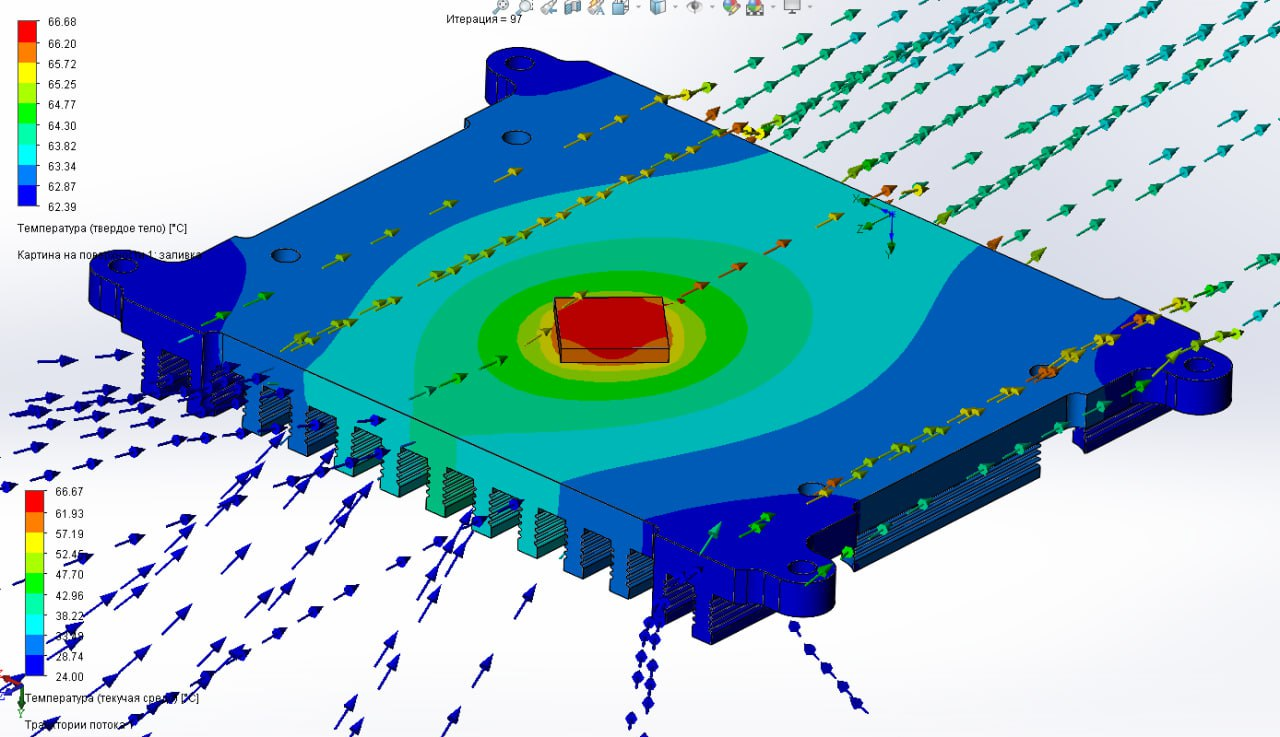
\includegraphics[width=0.8\textwidth]{heat.png}
    \caption{Расчет теплораспределения при 15 Вт потребления}
    \label{fig:heat_distribution}
\end{figure}

\section{Результаты}
В результате разработаны печатные платы для интерфейсов (рис. \ref{fig:interface_board}) и управляющего модуля ПЛК (рис. \ref{fig:plc_board}).

\begin{figure}
    \centering
    \begin{subfigure}{0.45\textwidth}
        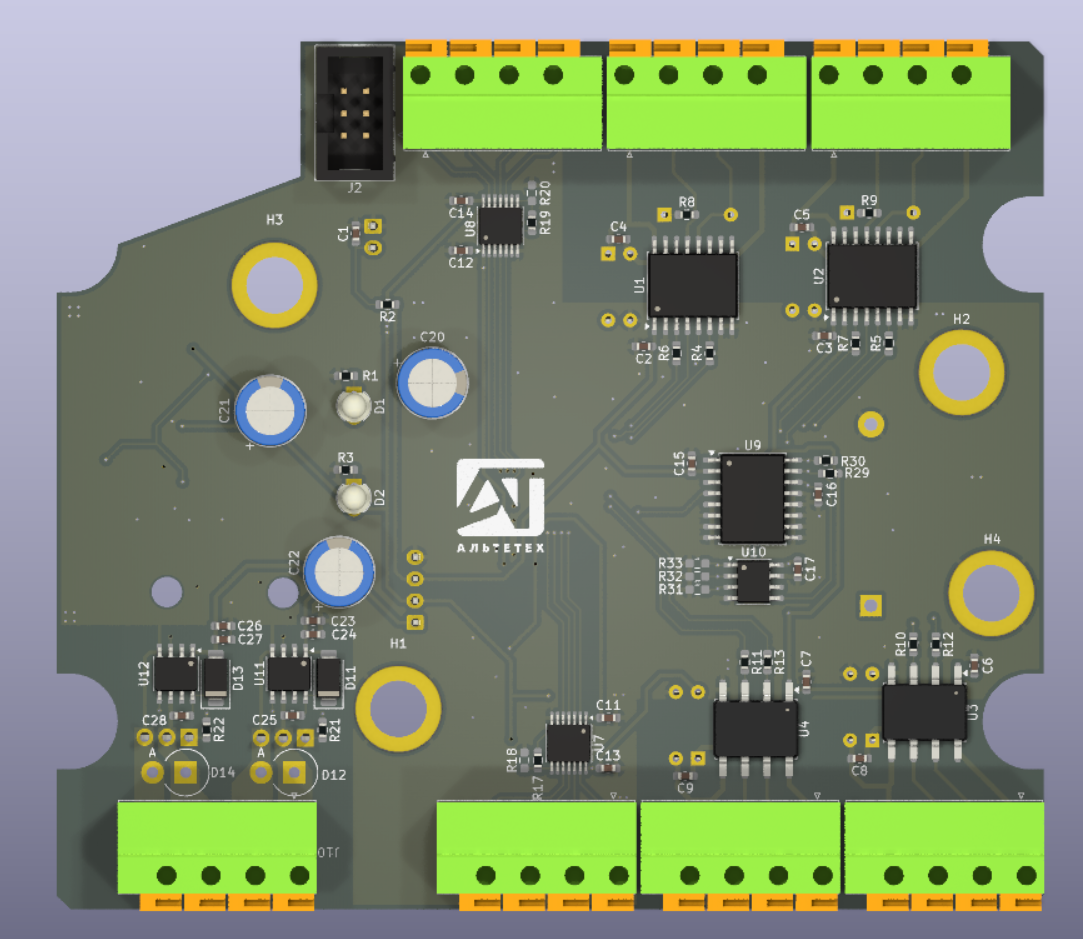
\includegraphics[width=\textwidth]{interface.png}
        \caption{Плата-расширения интерфейсов}
        \label{fig:interface_board}
    \end{subfigure}
    \hfill
    \begin{subfigure}{0.45\textwidth}
        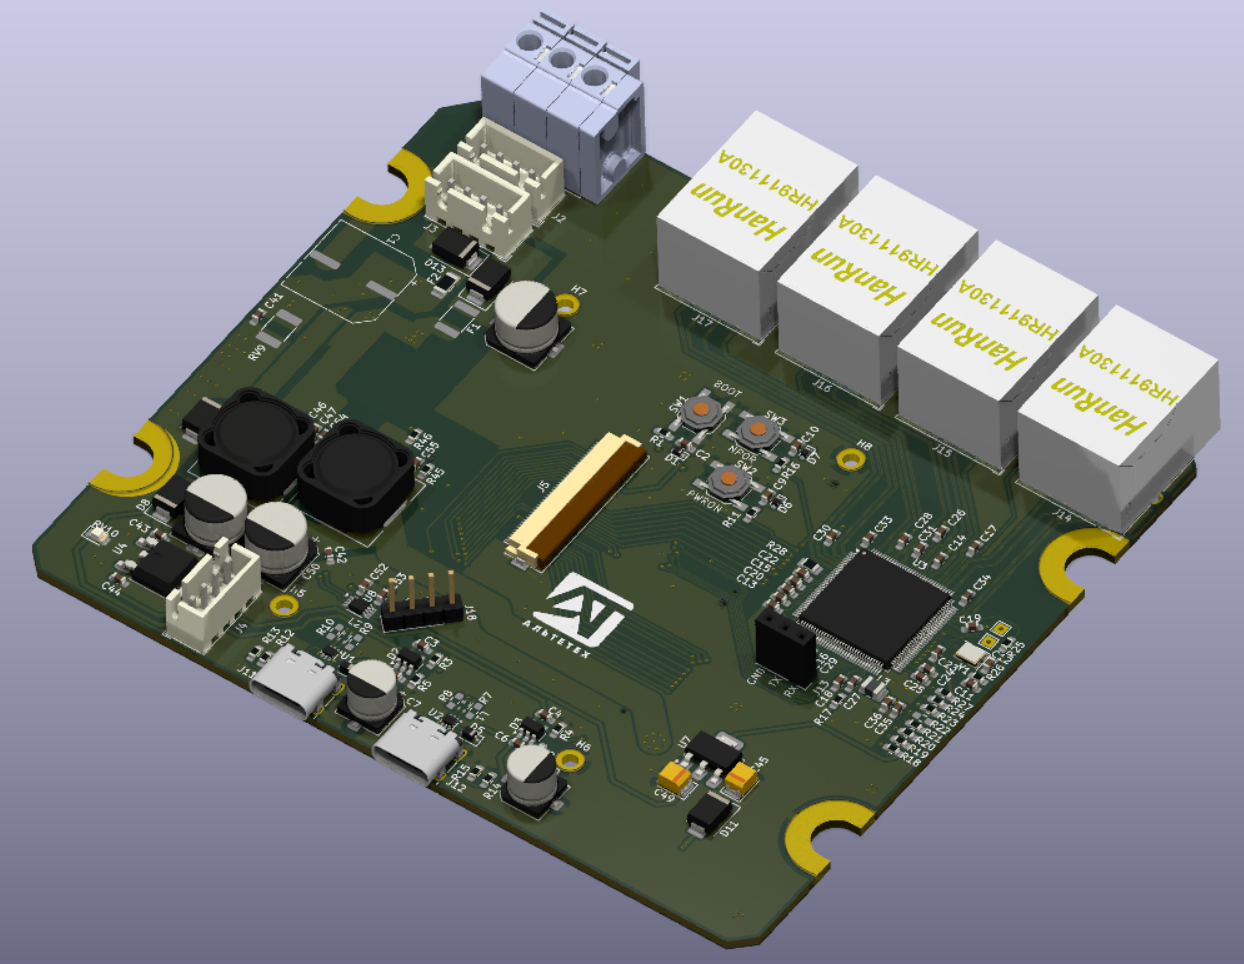
\includegraphics[width=\textwidth]{control.png}
        \caption{Плата управляющего модуля}
        \label{fig:plc_board}
    \end{subfigure}
    \caption{Разработанные печатные платы}
\end{figure}


\begin{figure}
    \centering
    \begin{subfigure}{0.45\textwidth}
        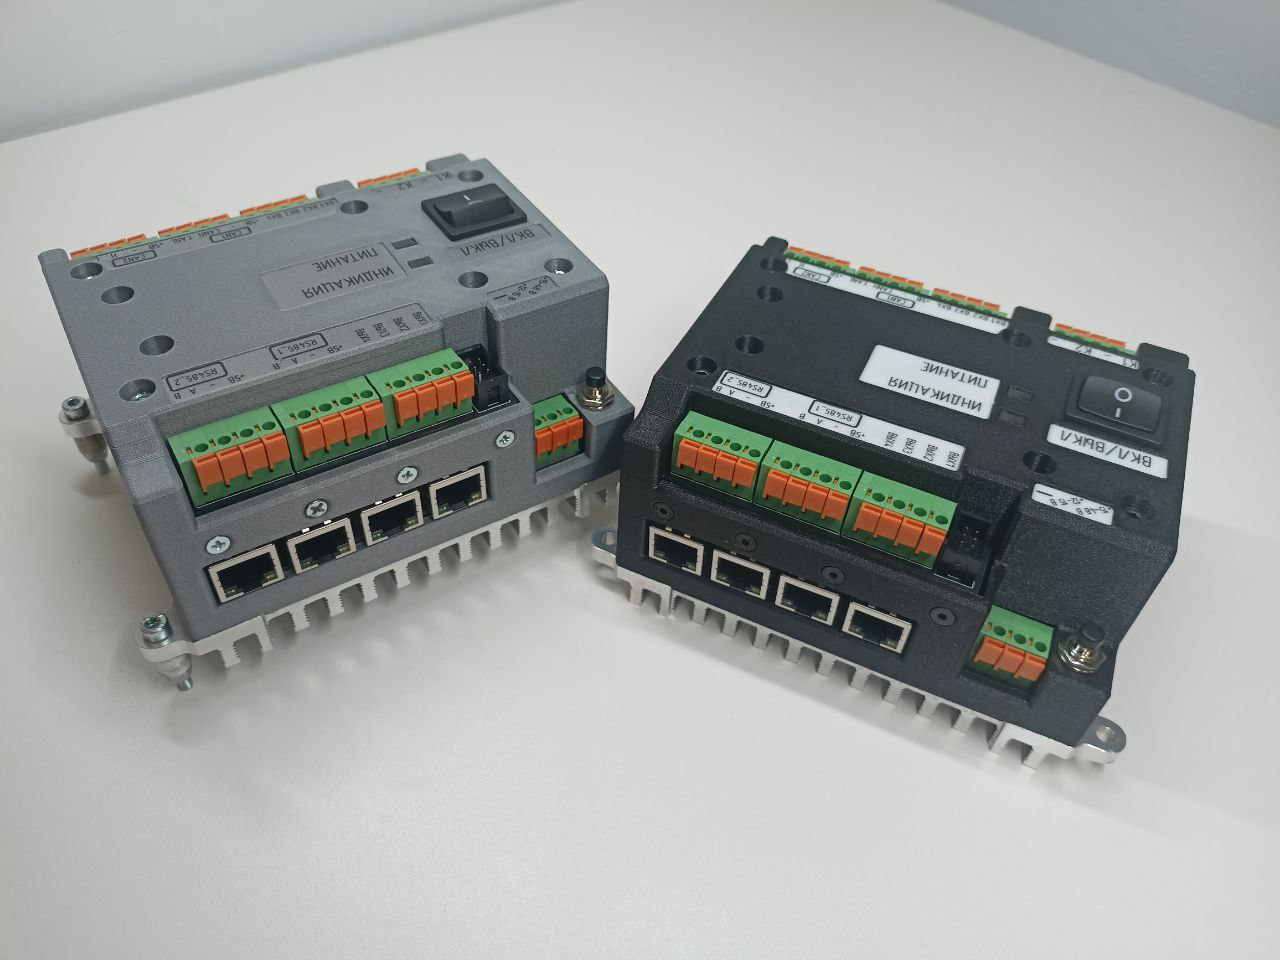
\includegraphics[width=\textwidth]{solution.png}
        \caption{Изделие в сборе}
    \end{subfigure}
    \hfill
    \begin{subfigure}{0.45\textwidth}
        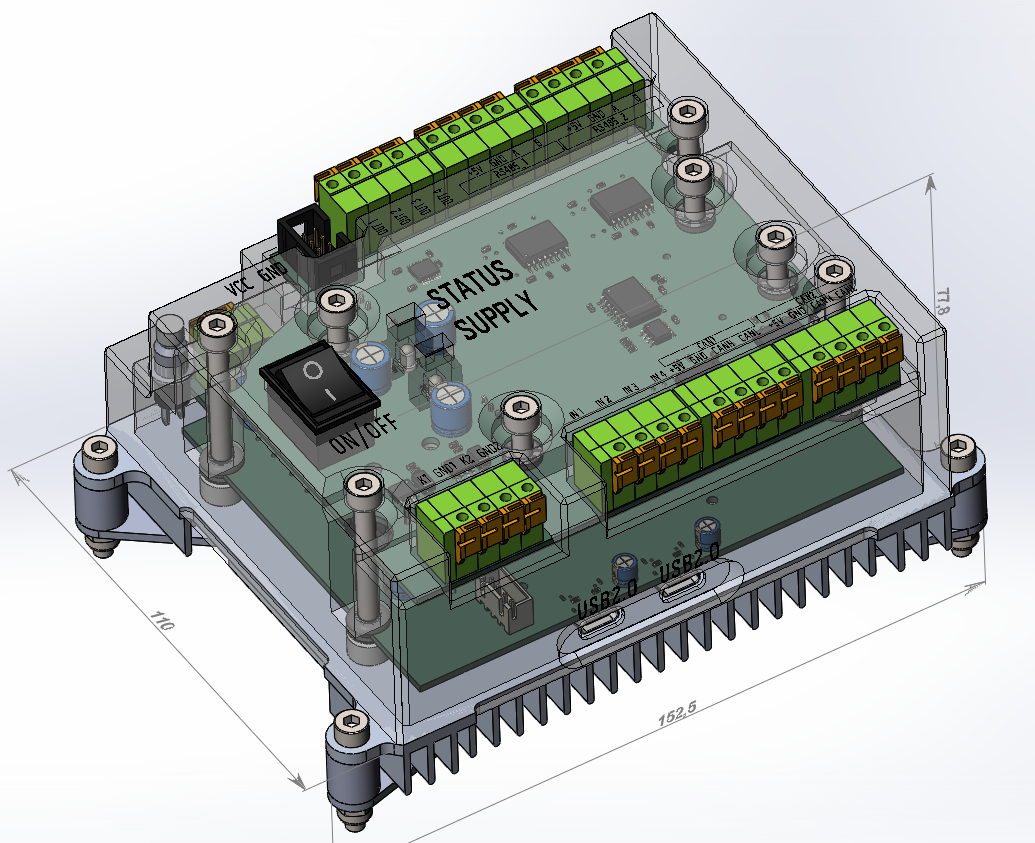
\includegraphics[width=\textwidth]{model.png}
        \caption{3D-модель}
        \label{fig:plc_board}
    \end{subfigure}
    \caption{}
\end{figure}

\section{Заключение}
Разработанная аппаратная платформа демонстрирует эффективность интеграции нейросетевых моделей в промышленные системы. Исключение промежуточных узлов позволило уменьшить задержки, повысить надежность и облегчить процесс масштабирования.

\newpage
\begin{thebibliography}{9}
\bibitem{ref1} Толстель О. В., Ширкин А. Е., Калабин А. Л. Построение системы технического зрения для выравнивания содержимого упаковок дельта-манипулятором на пищевом производстве // Программные продукты и системы. – 2023. – Т. 36. – №. 2. – С. 334-341.
\bibitem{ref2} Volkov A. K., Mironova L. V., Potapova S. E. The use of pretrained neural networks for solving the problem of reverse searching of X-ray images of prohibited items and substances // МГТУ ГА. – С. 9.
\bibitem{ref3} Мокрецов Н. С., Татарникова Т. М. Оптимизация процесса обучения при ограниченном объеме вычислительных ресурсов.
\bibitem{ref4} Степаненко С. О., Якимов П. Ю. Использование высокопроизводительной платформы глубокого обучения для ускорения обнаружения объектов // СБОРНИК ТРУДОВ ИТНТ-2019. – 2019. – С. 624-630.
\bibitem{ref5} Kortli Y. et al. Deep embedded hybrid CNN–LSTM network for lane detection on NVIDIA Jetson Xavier NX // Knowledge-based systems. – 2022. – Т. 240. – С. 107941.
\bibitem{ref6} Ismagilov R. Performance Evaluation of the Rockchip Systems-on-Chip Through YOLOv4 Object Detection Model // 2023 IEEE Ural-Siberian Conference on Biomedical Engineering, Radioelectronics and Information Technology (USBEREIT). – IEEE, 2023. – С. 241-243.
\bibitem{ref7} Савиных А. А., Астахов А. М. Прочностной и термодинамический расчет теплообменника // ББК 1 Н 34. – С. 5247.
\bibitem{ref8} Тестоедов Н. А. и др. Контроль зазоров в конструкциях технических изделий в процессе вибрационных испытаний // Обработка металлов: технология, оборудование, инструменты. – 2021. – Т. 23. – №. 2. – С. 40-53.
\bibitem{ref9} Ibrahim M. Q. et al. Optimizing Convolutional Neural Networks: A Comprehensive Review of Hyperparameter Tuning Through Metaheuristic Algorithms // Archives of Computational Methods in Engineering. – 2025. – С. 1-38.
\end{thebibliography}

\end{document}
